\section{Desarrollo}
\subsection{Teoría}
Para lograr los efectos necesarios, las coordenas de la imagen original deben ser modificadas mediante una transformación lineal seguida de una traslación (lo que comúnmente se conoce como \textit{transformación afín}).

\par La transformación utilizada puede verse en la figura~\ref{fig:transformacion1}. Los valores $a, b, c, d$ son los coeficiententes de transformación, $(x ,y)$ son las coordenadas originales, $x_{0}$ e $y_{0}$ son el offset y $x$', $y$' son las coordenadas resultantes.     

\begin{figure}[h!]
 \caption{Transformación utilizada}
 \centering
   $
   \begin{bmatrix}
x'\\y' 

\end{bmatrix}
=
\begin{bmatrix}
 a & b  & x_{0} \\ 
 a & b  & y_{0} 
\end{bmatrix}
\begin{bmatrix}
x - x_{0}\\ 
y - y_{0}\\
1 
\end{bmatrix}
   $
\end{figure}

En nuestro caso, los coeficientes de transformación deben ser configurados para que la ecuación quede como en la figura~\ref{fig:transformacion2} 

\begin{figure}[h!]
 \caption{Transformación con los coeficientes}
 \centering
 $
 \begin{bmatrix}
x'\\y' 

\end{bmatrix}
=
   \begin{bmatrix}
 \cos \alpha & \sin\alpha  & x_{0} \\ 
 -\sin \alpha & \cos\alpha  & y_{0} 
\end{bmatrix}
\begin{bmatrix}
x - x_{0}\\ 
y - y_{0}\\
1 
\end{bmatrix}
$
   \label{fig:transformacion2}
\end{figure}

\subsection{Detalles de la implementación}
\subsubsection{Utilización de memoria}
Uno de los primeros problemas a solucionar fue cómo calcular los valores de las funciones seno y coseno, ya que la fpga no posee una fpu. La solución consistió en guardar en dos tablas $360$ valores correspondientes a parámetros angulares para dichas funciones (de 0 a 359 grados). Cada resultado se guardó en 16 bits en forma signo más magnitud, con 7 bits para la parte entera y 8 para la decimal, lo que en total ocupó 720 bytes de memoria.
\par La imagen a cargar, por otro lado, es de 64 por 64 pixeles, y cada pixel tiene tres bits para el canal rojo, tres bits para el verde y dos para el azul. Esto resulta en un bitmap que tiene 4096 valores de 8 bits y ocupa en memoria 4096 bytes. En la figura~\ref{fig:chess} se puede observar el bitmap utilizado. 

\begin{figure}[h!]
 \caption{bitmap utilizado}
 \centering
   
\includegraphics[width=0.5\textwidth]{bitmap.png}
   \label{fig:chess}
\end{figure}   

\subsubsection{Paralelismo}
En la implementación de las operaciones matemáticas necesarias para resolver el problema consideramos oportuno utilizar lógica combinacional para mayor velocidad. De haber usado máquina de estados, la velocidad de ejecución habría sido bastante menor.

\subsubsection{Salida a video}
blablabla?

\subsubsection{Otros detalles}
blablabla?

\subsection{Arquitectura}
Podemos ver un esquema general en la figura~\ref{fig:arquitectura}
\begin{figure}[h!]
 \caption{Arquitectura general}
 \centering
   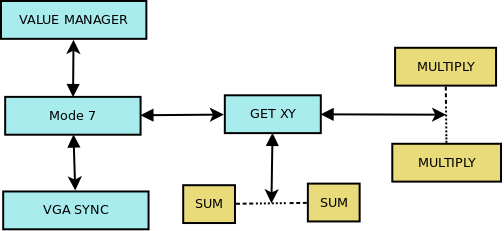
\includegraphics[width=0.75\textwidth]{arquitectura.png}
   \label{fig:arquitectura}
\end{figure} 

\begin{itemize}
\item \textbf{Mode 7} es el módulo central de la arquitectura, es decir, el encargado de hacer pedidos a los otros módulos y trasladar los resultados entre ellos. 
\item El módulo \textbf{Value Manager} es el encargado de interpretar las entradas de los switches y botones, que sirven para cambiar entre las distintas transformaciones de la imagen.
\item El módulo \textbf{Get XY} es el encargado de hacer operaciones sobre los pixeles, utilizando varias encarnaciones de los módulos \textbf{SUM} y \textbf{MULTIPLY}. Allí también se realiza el cargado de las tablas de seno, coseno y la imagen.
\item Finalmente, el módulo \textbf{VGA SYNC} es el encargado de la salida al monitor.
\end{itemize}